\section{Understanding the role of convolutions and pooling operations}\label{sec:conv}
In this section, we will use the frameworks of DGNs and ``path-view'' to obtain insights about (i) convolutional layers and (ii) pooling: global average pooling\footnote{The arguments can be extended to $\max$-pooling with technical modifications.}. In this section, we continue to be in the DGN setup, i.e., we will have separate parameterisations $\Tg$ and $\Tw$, and assume that Assumptions~\ref{assmp:mainone}, \ref{assmp:maintwo} hold. However, we impose additional restrictions to account for the presence of convolutional and pooling layers, which, we describe below.

\textbf{Circular Convolutional layers:}

$1.$ We assume that, the initial $0<L<d$ layers are convolutional layers. In particular, each layer uses a $1$-dimensional kernel of width $0<\hat{w}<d_{in}$, and the output of each layer is a $d_{in}$-dimensional vector.

$2.$ We consider circular convolutional operations instead of zero padding, i.e., during the convolution operation, say index $i$ exceeds $d_{in}$ then it will be considered as $i-d_{in}$, and in the case when a negative index is required, i.e., if index $i<0$ is needed, then $d_{in}+i$ will be used instead. We illustrate this circular convolution with the help of \Cref{fig:circconv}, wherein, $\hat{w}=2$, $d_{in}=3$. Here, $\theta^{(l)}(i),l=1,\ldots,L-1, i=1,2$ are the weights, and the final layer weight $\theta^{(L)}=\left[\frac{1}{d_{in}},\ldots, \frac{1}{d_{in}}\right]^\top\in \R^{d_{in}}$ in the case of global average pooling. Note that, in \Cref{fig:circconv}, we have used only one network, and we have also used a simpler and different notation for the weights: this is because, in DGN (with circular convolutions), both the gating network parameterised by $\Tg$ and the weights network parameterised by $\Tw$ will have identical architecture, and in order to explain just the circular convolution alone more clearly, we have used a simpler notation for the weights and have left the gating information unspecified in \Cref{fig:circconv}.

\begin{figure}
\centering
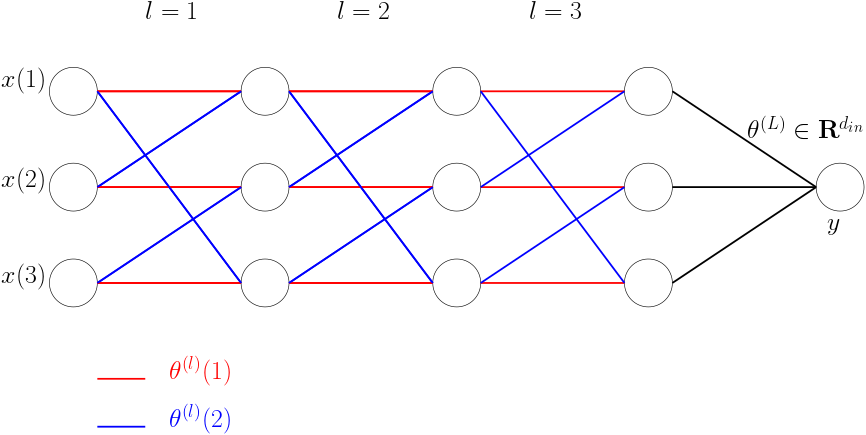
\includegraphics[scale=0.25]{figs/circconv.png}
\caption{Shows a circular convolutional network with $d_{in}=3$ and kernel size $\hat{w}=2$. Note that there are only $8$ unique path strengths in this example (in the case of global average pooling).}
\label{fig:circconv}
\end{figure}



\textbf{Path Sharing:} With the understanding of circular convolution in the background, we now investigate the similarity of two inputs $x_s\in \R^{d_{in}}$ and $x_{s'}\in \R^{d_{in}}$ after they pass through $L$ convolutional layers. To be specific, let $x_s(L)\in \R^{d_in}$ and $x_{s'}(L)\in \R^{d_{in}}$ be the outputs obtained after the $L$ convolutional layers. Note that $x_s(L)=(x_s(L,i),i\in[d_{in}])\in \R^w$ is a $d_{in}$-dimensional vector with $i=1,\ldots,d_{in}$ components, wherein, the $i^{th}$ component is obtained by circular convolution using a kernel of size $0<\hat{w}<d_{in}$. Further, we restrict our attention to the first $L$ layers which perform the convolution operations. We are interested in investigating the following: 
\begin{align}
\E{\ip{x_s(L),x_{s'}(L) }}=\sum_{i=1}^{d_{in}} \E{x_s(L,i)x_{s'}(L,i)}
\end{align}
Given the randomised and symmetric nature of the weight initialisation, without loss of generality, it is sufficient to study $\E{x_s(L,1)x_{s'}(L,1)}$, i.e., it is enough to consider the case of $L$ convolutions with kernel of size $\hat{w}$ followed by a global average pooling. We now make the following observations:

$1.$ There are $p=1,\ldots,\hat{P}=d_{in}\hat{w}^{d-1}$ paths.

$2.$ There are $k=1,\ldots,\hat{B}=\hat{w}^{d-1}$ unique path strengths. This is due to the fact that the same path strength repeats $d_{in}$ times. For instance, in \Cref{fig:circconv}, the path strength $\theta^{1}(1)\theta^{1}(2)\theta^{1}(3)\frac{1}{d_{in}}$ repeats $3$ times.

$3.$ Paths can be grouped into bundles $b_k,k\in[\hat{w}^{d-1}]$, wherein, bundle $b_k$ comprises of $d_{in}$ paths, all of which have the same path strength. Without loss of generality, $b_k$ comprises of paths $(k-1)d_{in}+1,\ldots, kd_{in}$.

$4.$ The path strength $w_t=(w_t(b_1),\ldots, w_t(b_{\hat{B}}))\in \R^{\hat{P}}$, where $w_t(b_k)=(w_t(p),p=(k-1)d_{in}+1,\ldots,kd_{in})\in \R^{d_{in}}$. 

$5.$ The output $x_s(L,1)=\phi^\top_{x_s,\G_t} w_t$.

\begin{lemma}\label{lm:invariance}
At $t=0$, under Assumptions~\ref{assmp:mainone},\ref{assmp:maintwo}, convolutional layers with global average pooling at the end causes translational invariance.
\begin{align*}
&\E{x_s(L,1)x_{s'}(L,1)}\\&=\frac{\sigma^{2(d-1)}}{d^2_{in}}\sum_{k=1}^{\hat{B}} \sum_{p_1,p_2\in b_k}  \Big( x(p_1(0),s) A(x_s,p_1)\\
&\quad\quad \quad\quad \quad\quad x(p_2(0),s') A(x_{s'},p_2) \Big)
\end{align*}
\end{lemma}

\textbf{Remark:} Now, for $i\in\{0,\ldots, d_{in}-1\}$, let $z^{(i)}\in \R^{d_{in}}$ be the clockwise rotation of $z\in \R^{d_{in}}$ by $i$ co-ordinates, and let $x^{(i)}\in \R^{d_{in}\times n}$ be the data matrix obtained by clockwise rotation of the columns of the data matrix $x\in \R^{d_{in}\times n}$ by $i$ co-ordinates. Then, we have

\begin{align*}
&\E{x_s(L,1)x_{s'}(L,1)}\\
&=\frac{\sigma^{2(d-1)}}{d^2_{in}}\sum_{k=1}^{\hat{B}} \sum_{i=1}^{d_{in}} \sum_{p\in b_k}   \Big(x(p(0),s) A(x,p) \\ 
&\quad\quad \quad\quad \quad\quad x^{(i)}(p(0),s') A(x^{(i)}_{s'},p) \Big)
\end{align*}
The term $\sum_{p\in b_k}  x(p(0),s) A(x,p) x^{(i)}(p(0),s') A(x^{(i)}_{s'},p)$ is translation invariant.


\begin{comment}
\textbf{Claim $2$:} At $t=0$, under Assumptions~\ref{assmp:mainone},\ref{assmp:maintwo}, convolutional layers with $\max$-pooling at the end causes translational invariance.

\begin{proof}
The proof follows in a manner similar to \textbf{Claim $1$} made for the case of global average pooling. However, the technical challenge is the following: in the case of $\max$-pooling, only one of the $d_{in}$ paths connecting the $(L-1)^{th}$ layer to the output node is \emph{on}. This path connects the ``$\max$" node in the $(L-1)^{th}$ layer to the output node. This can be accounted in the calculations by setting the path strength to be $0$ for those paths that do not pass through the ``$\max$" node in the $(L-1)^{th}$ layer.  We make the following observations about $M$:

$1.$ For each bundle $b_k, k\in[\hat{B}]$, $\exists$ unique indices $i(k), j(k)\in [d_{in}]$ such that $M((k-1)d_{in}+i(k), (k-1)d_{in}+j(k))=\sigma^{2(d-1)}$, and rest of the entries of $M$ are $0$.

$2.$ $M(p_1,p_2)=\frac{\sigma^{2(d-1)}}{d^2_{in}}$, if $p_1$ and $p_2$ belong to the same bundle continues to hold trivially due to observation $1$ (of the current claim).

And by going through reductions similar to \textbf{Claim $1$}, we have

\begin{align*}
&\E{x_s(L,1)x_{s'}(L,1)}\\&=\phi^\top_{x_s,\G_0} M \phi^\top_{x_{s'},\G_0}\\
&=\sum_{p_1,p_2=1}^{\hat{P}} \Big(x(p_1(0),s) A(x_s,p_1) \\
&\quad\quad \quad\quad \quad\quad x(p_2(0),s') A(x_{s'},p_2) M(p_1,p_2)\Big)\\
&=\frac{\sigma^{2(d-1)}}\sum_{k=1}^{\hat{B}} \sum_{p_1,p_2\in b_k}  \Big( x(p_1(0),s) A(x_s,p_1)\\
&\quad\quad \quad\quad \quad\quad x(p_2(0),s') A(x_{s'},p_2) \Big)
\end{align*}
Now, for $i\in\{0,\ldots, d_{in}-1\}$, let $z^{(i)}\in \R^{d_{in}}$ be the clockwise rotation of $z\in \R^{d_{in}}$ by $i$ co-ordinates, and let $x^{(i)}\in \R^{d_{in}\times n}$ be the data matrix obtained by clockwise rotation of the columns of the data matrix $x\in \R^{d_{in}\times n}$ by $i$ co-ordinates. Then, we have

\begin{align*}
&\E{x_s(L,1)x_{s'}(L,1)}\\
&=\frac{\sigma^{2(d-1)}}{d^2_{in}}\sum_{k=1}^{\hat{B}} \sum_{i=1}^{d_{in}} \sum_{p\in b_k}   \Big(x(p(0),s) A(x,p) \\ 
&\quad\quad \quad\quad \quad\quad x^{(i)}(p(0),s') A(x^{(i)}_{s'},p) \Big)
\end{align*}
The term $\sum_{p\in b_k}  x(p(0),s) A(x,p) x^{(i)}(p(0),s') A(x^{(i)}_{s'},p)$ is translation invariant.

\end{proof}
\end{comment}